% Editable README artwork; schematic contacts, not measurements or a benchmark.
% Render: latexmk -pdf -jobname=tcren-splash-light tcren-splash.tex
% Dark: latexmk -pdf -jobname=tcren-splash-dark tcren-splash.tex
% Export with pdftocairo -svg input.pdf output.svg; PNG fallback: rsvg-convert -w 1800 input.svg -o output.png.
\documentclass[border=0pt]{standalone}
\usepackage{tikz,amsmath,amssymb,helvet}
\usetikzlibrary{arrows.meta,calc}
\renewcommand{\familydefault}{\sfdefault}
\ifnum\pdfstrcmp{\jobname}{tcren-splash-dark}=0\def\darkmode{1}\fi
\ifdefined\darkmode
  \definecolor{paper}{HTML}{101B27}\definecolor{ink}{HTML}{E6EFF7}
  \definecolor{muted}{HTML}{A5B7C9}\definecolor{rule}{HTML}{42576A}
  \definecolor{energy}{HTML}{ED9DC6}\definecolor{conf}{HTML}{73BAEA}
  \definecolor{betti}{HTML}{E5BC58}\definecolor{motif}{HTML}{65D1BD}
\else
  \definecolor{paper}{HTML}{F7FAFC}\definecolor{ink}{HTML}{193248}
  \definecolor{muted}{HTML}{5C7489}\definecolor{rule}{HTML}{BDCCD7}
  \definecolor{energy}{HTML}{AF477C}\definecolor{conf}{HTML}{267CB2}
  \definecolor{betti}{HTML}{A57709}\definecolor{motif}{HTML}{128779}
\fi
\pagecolor{paper}\color{ink}
\begin{document}
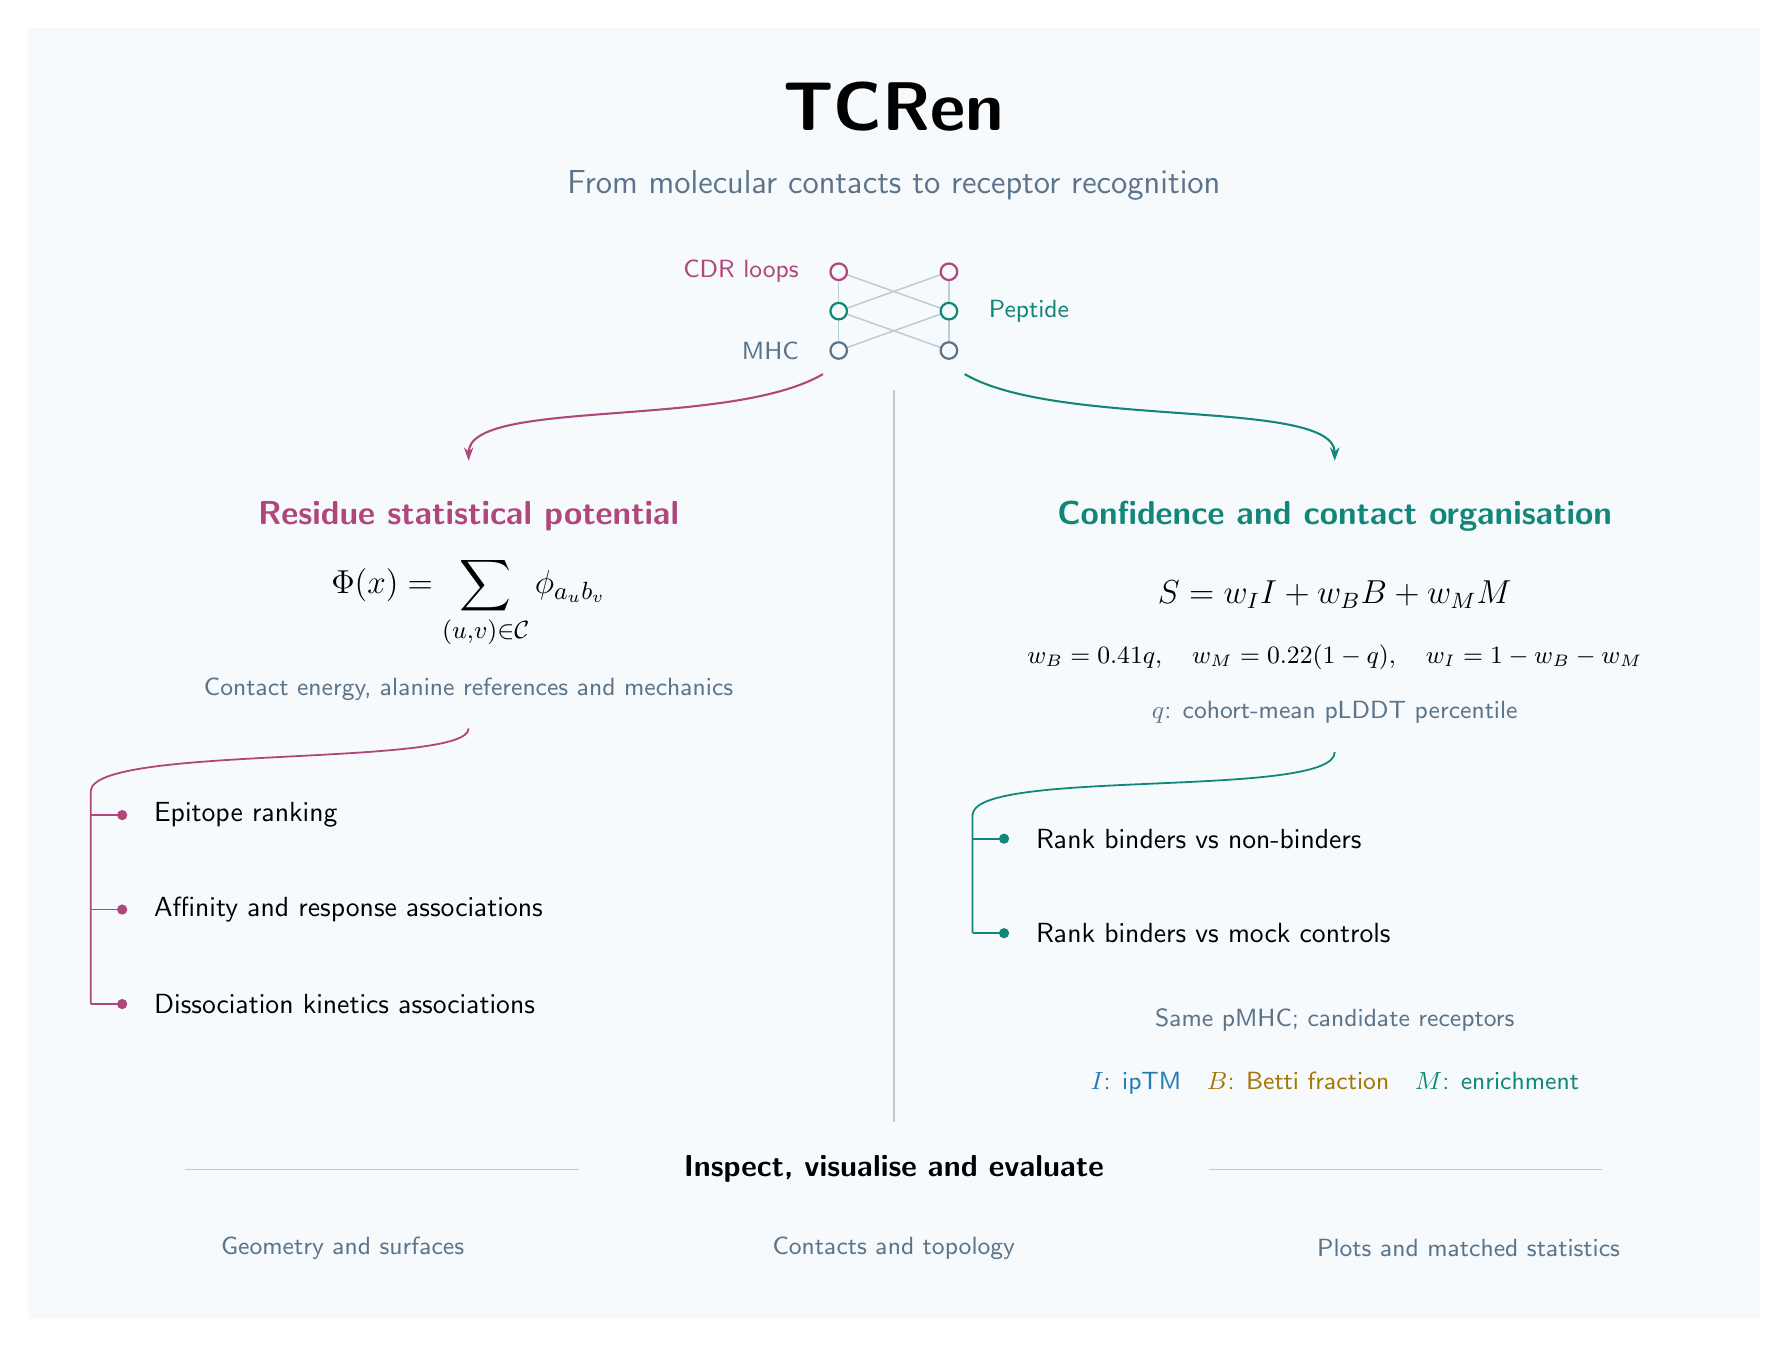
\begin{tikzpicture}[x=1mm,y=1mm,
 every node/.style={font=\fontsize{10}{12}\selectfont,inner sep=0pt},
 title/.style={font=\bfseries\fontsize{24}{28}\selectfont},
 route/.style={font=\bfseries\fontsize{13}{16}\selectfont},
 sub/.style={font=\fontsize{9}{11}\selectfont,text=muted},
 flow/.style={line width=.75pt,-{Stealth[length=1.7mm,width=1.2mm]}},
 branch/.style={line width=.65pt},
 atom/.style={circle,minimum size=2.1mm,inner sep=0pt,fill=paper,line width=.8pt}]
\useasboundingbox (0,0) rectangle (220,-164);
\fill[paper] (0,0) rectangle (220,-164);
\node[title] at (110,-10) {TCRen};
\node[text=muted,font=\fontsize{12}{15}\selectfont] at (110,-20)
 {From molecular contacts to receptor recognition};
% One schematic graph supplies chemistry, topology and inspection.
\begin{scope}[shift={(110,-36)}]
 \foreach \a/\b in {1/3,1/4,2/3,2/4,3/5,3/6,4/5,4/6,1/5,2/6}
  {\coordinate (p1) at (-7,5);\coordinate (p2) at (7,5);
   \coordinate (p3) at (-7,0);\coordinate (p4) at (7,0);
   \coordinate (p5) at (-7,-5);\coordinate (p6) at (7,-5);
   \draw[rule,line width=.55pt] (p\a)--(p\b);}
 \foreach \n in {1,2}{\node[atom,draw=energy] at (p\n) {};}
 \foreach \n in {3,4}{\node[atom,draw=motif] at (p\n) {};}
 \foreach \n in {5,6}{\node[atom,draw=muted] at (p\n) {};}
 \node[sub,anchor=east,text=energy] at (-12,5) {CDR loops};
 \node[sub,anchor=west,text=motif] at (12,0) {Peptide};
 \node[sub,anchor=east] at (-12,-5) {MHC};
\end{scope}
\draw[flow,energy] (101,-44) .. controls (89,-51) and (56,-47) .. (56,-55);
\draw[flow,motif] (119,-44) .. controls (131,-51) and (166,-47) .. (166,-55);
\draw[rule,branch] (110,-46)--(110,-139);
% The two routes have different tasks and different scientific interpretations.
\node[route,text=energy] at (56,-62) {Residue statistical potential};
\node[font=\fontsize{13}{16}\selectfont] at (56,-73)
 {$\displaystyle\Phi(x)=\sum_{(u,v)\in\mathcal C}\phi_{a_u b_v}$};
\node[sub] at (56,-84) {Contact energy, alanine references and mechanics};
\draw[energy,branch] (56,-89) .. controls (56,-94) and (8,-91) .. (8,-97) -- (8,-124);
\foreach \y in {-100,-112,-124}{\draw[energy,branch] (8,\y)--(12,\y);}
\foreach \y in {-100,-112,-124}{\fill[energy] (12,\y) circle (.65mm);}
\node[anchor=west] at (16,-100) {Epitope ranking};
\node[anchor=west] at (16,-112) {Affinity and response associations};
\node[anchor=west] at (16,-124) {Dissociation kinetics associations};
\node[route,text=motif] at (166,-62) {Confidence and contact organisation};
\node[font=\fontsize{12}{15}\selectfont] at (166,-72)
 {$S=w_I I+w_B B+w_M M$};
\node[font=\fontsize{9}{11}\selectfont] at (166,-80)
 {$w_B=0.41q,\quad w_M=0.22(1-q),\quad w_I=1-w_B-w_M$};
\node[sub] at (166,-87) {$q$: cohort-mean pLDDT percentile};
\draw[motif,branch] (166,-92) .. controls (166,-98) and (120,-94) .. (120,-100) -- (120,-115);
\foreach \y in {-103,-115}{\draw[motif,branch] (120,\y)--(124,\y);}
\foreach \y in {-103,-115}{\fill[motif] (124,\y) circle (.65mm);}
\node[anchor=west] at (128,-103) {Rank binders vs non-binders};
\node[anchor=west] at (128,-115) {Rank binders vs mock controls};
\node[sub] at (166,-126) {Same pMHC; candidate receptors};
% Colour carries the component identity, without implying independent evidence.
\node[font=\fontsize{9}{11}\selectfont] at (166,-134)
 {{\color{conf}$I$: ipTM}\quad {\color{betti}$B$: Betti fraction}\quad {\color{motif}$M$: enrichment}};
\node[font=\bfseries\fontsize{11}{14}\selectfont,fill=paper,inner xsep=3mm] at (110,-145)
 {Inspect, visualise and evaluate};
\draw[rule,branch] (20,-145)--(70,-145);
\draw[rule,branch] (150,-145)--(200,-145);
\node[sub] at (40,-155) {Geometry and surfaces};
\node[sub] at (110,-155) {Contacts and topology};
\node[sub] at (183,-155) {Plots and matched statistics};
\end{tikzpicture}
\end{document}
